%Nama Kelompok: Kernel
%Kelas: D4 1B
%Anfhaz Grady Octavavian 1174048
%Dika Sukma Pradana 1174050
%Ikhsan Al Azis 1174049
%Rangga Putra 1174056
%Surya Pandu 1174036
%Syahriyan Zulfani 1174037
%Teddy Gideon Manik 1174038

	
	\section{Kernel}
Kernel merupakan sebuah perangkat lunak yang menjadi bagian utama dlam sebuah system operasi computer, yaitu untuk membantu macam-macam program aplikasi untuk mengakses hardware. 
Dengan kata lain, kernel adalah mediator antara software dan hardware yang menyediakan pengaturan input-output, pengaturan fila dan yang lainnya. 
Yang sering kita kenal itu adalah kernel linux. Pengertian secara garis besarnya sama saja. Kernel linux ini penemunya yaitu  murid Ilmu Komputer berkebangsaan Finlandia, Linus Torvalds pada tahun 1991.

	 Kernel adalah program komputer yang merupakan inti dari sistem operasi komputer, dengan kontrol penuh atas segala hal yang ada di sistem. Pada kebanyakan sistem, ini adalah salah satu program pertama yang dimuat
	 saat start-up (setelah bootloader). 
	 Ini menangani sisa start-up serta permintaan input / output dari perangkat lunak, menerjemahkannya ke dalam instruksi pengolahan data untuk unit pemrosesan pusat. Ini menangani memori dan periferal seperti keyboard, 
	 monitor, printer, dan speaker.
	 Kernel menghubungkan perangkat lunak aplikasi ke perangkat keras komputer.
	 Kode kritis kernel biasanya dimuat ke dalam area lindung memori, yang mencegahnya ditimpa oleh aplikasi atau komponen lain yang lebih kecil dari sistem operasi. Kernel menjalankan tugasnya, seperti menjalankan proses 
	 dan penanganan interupsi, di dalam ruang kernel. 
	 Sebaliknya, semua yang dilakukan pengguna ada di ruang pengguna, menulis teks di editor teks, menjalankan program di GUI, dll. Pemisahan ini mencegah data pengguna dan data kernel tidak saling mengganggu dan menyebabkan 
	 ketidakstabilan dan kelambatan. 
	 Antarmuka kernel adalah lapisan abstraksi tingkat rendah. Ketika sebuah proses membuat permintaan dari kernel, itu disebut system call. Desain kernel berbeda dalam cara mereka mengatur panggilan dan sumber sistem ini. 
	 Kernel monolitik menjalankan semua instruksi sistem operasi di ruang alamat yang sama untuk kecepatan. Sebuah mikrokernel menjalankan sebagian besar proses di ruang pengguna, untuk modularitas. 
	
	contoh gambar kernel \ref{kernel}

	\begin{figure}[ht]
		\centerline{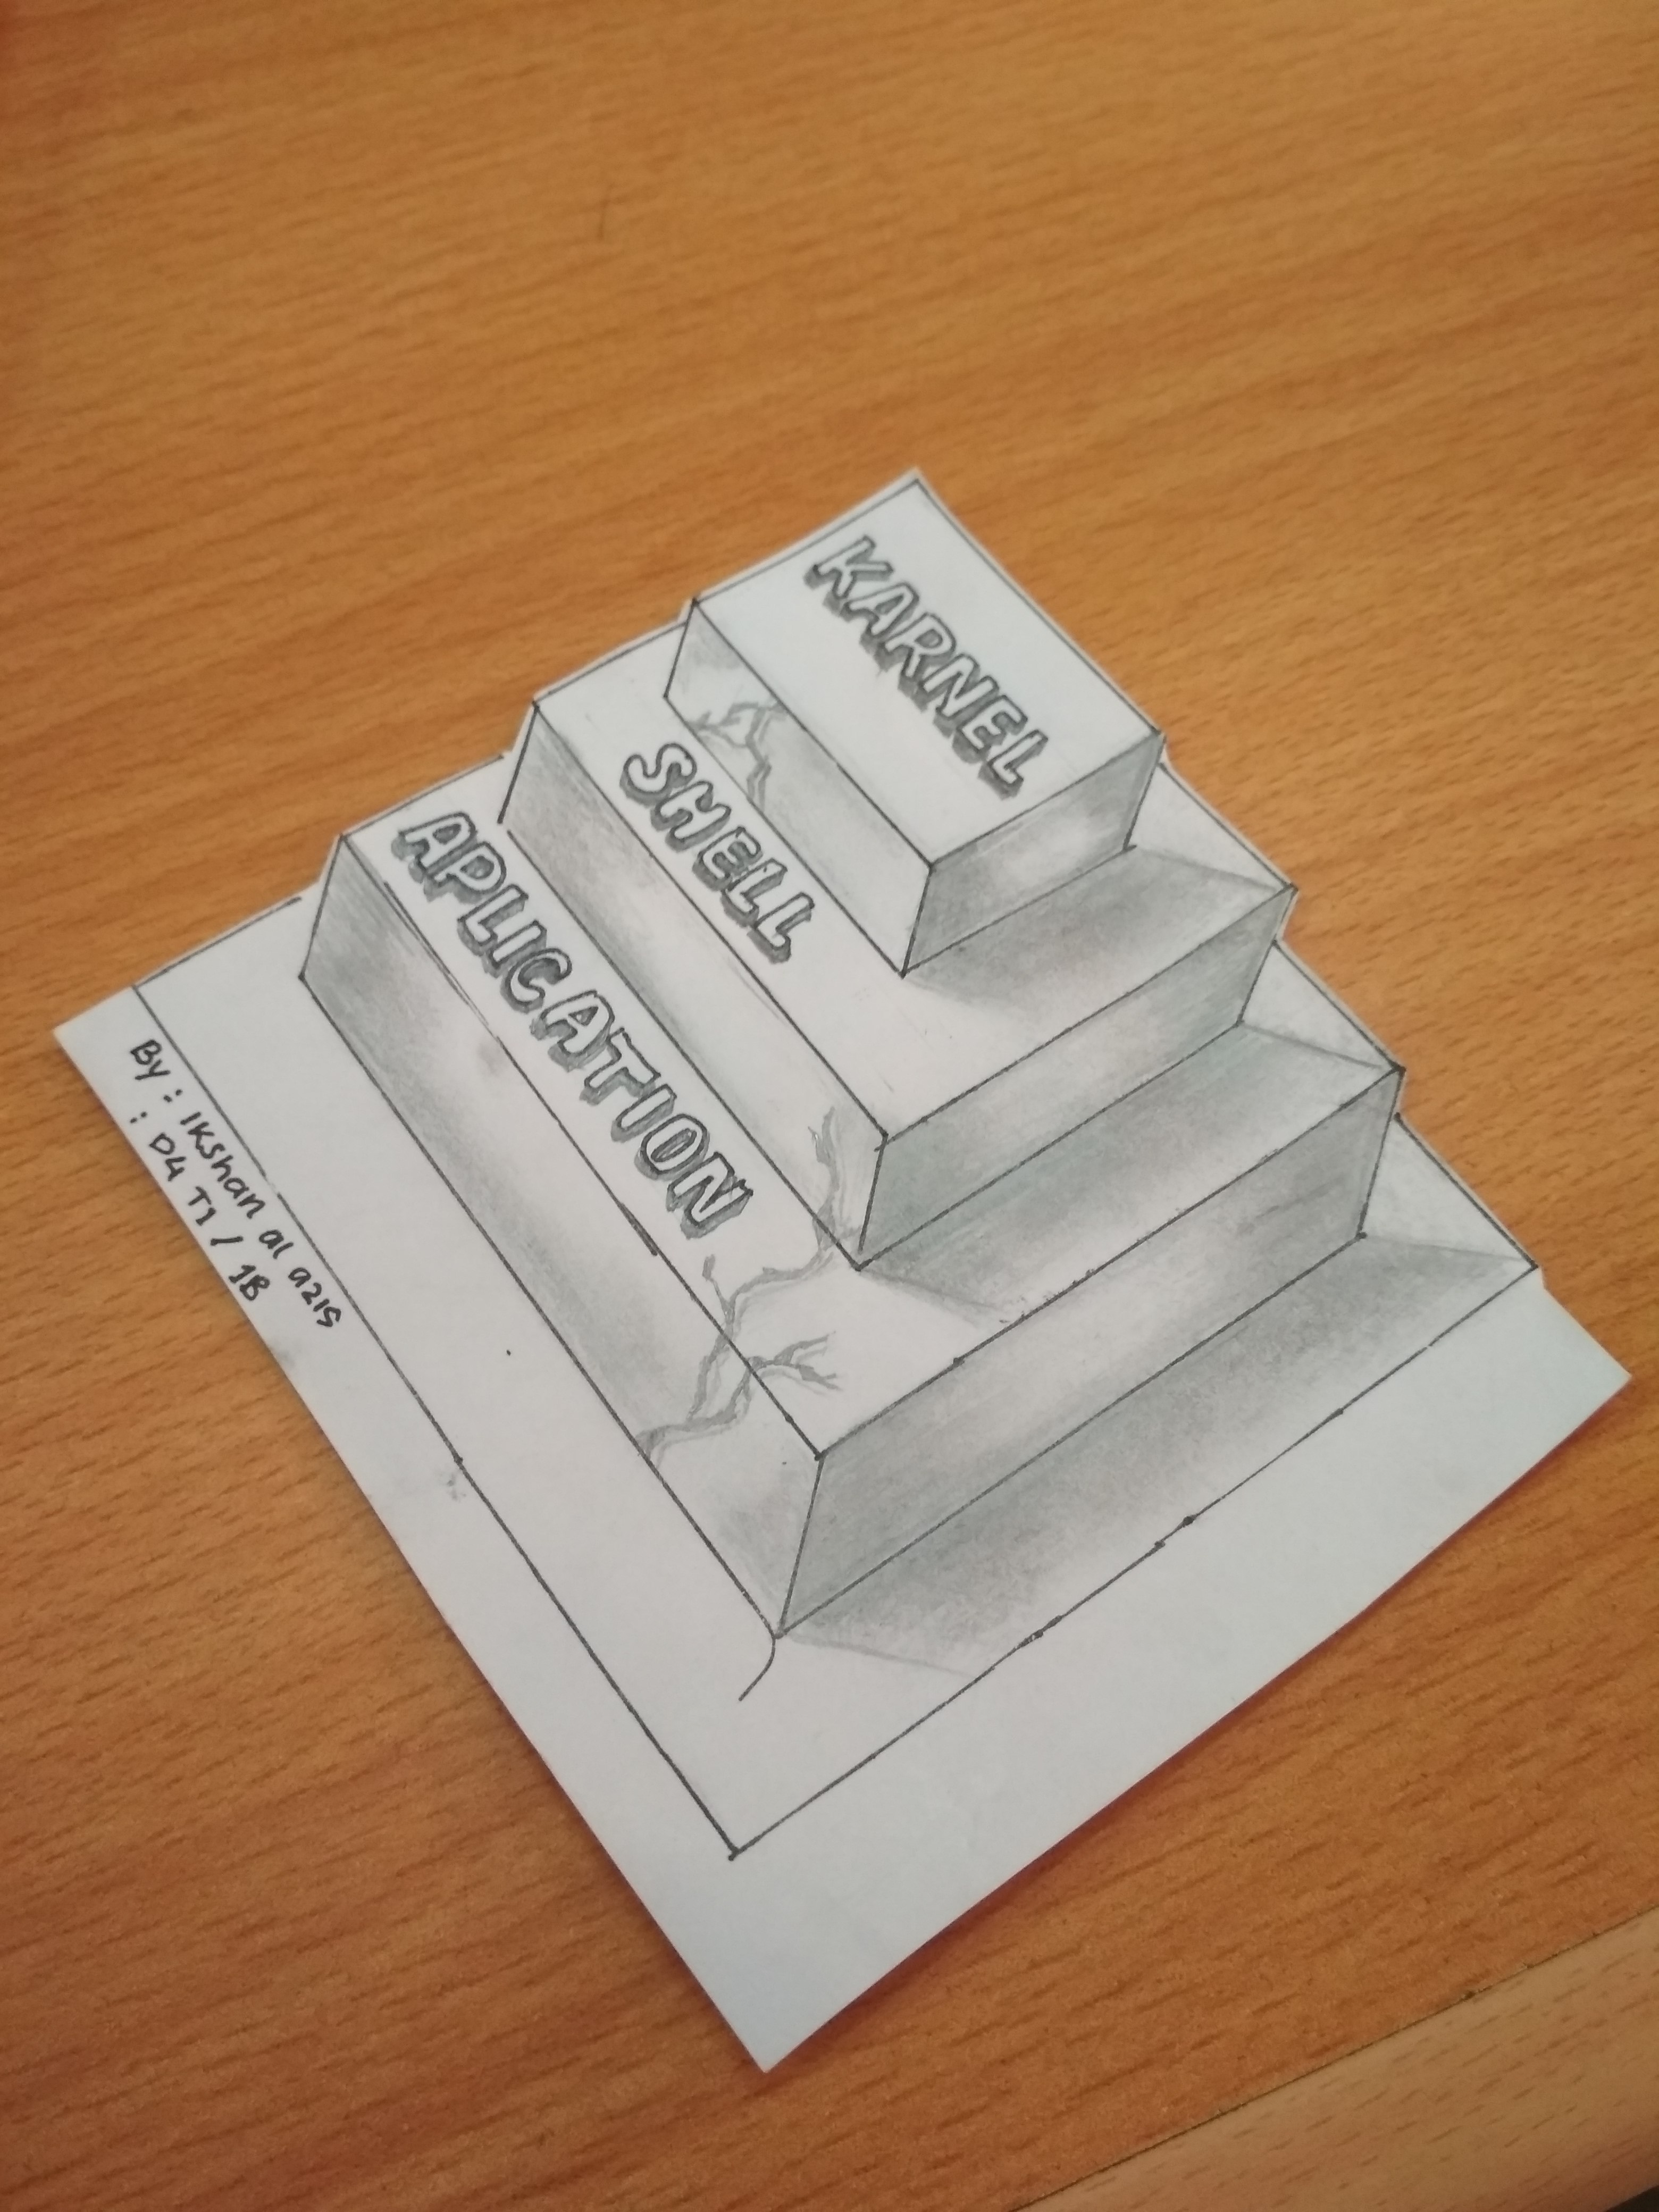
\includegraphics[width=1\textwidth]{figures/Kernel.jpg}}
		\caption{gambar kernel.}
		\label{kernel}
	\end{figure}

		\subsection{Sejarah Kernel}
		 Kernel merupakan program komputer yang mengatur semua permintaan akan input/output dari perangkat lunak atau software.
		 Pada tahun 1990an, sebuah jenis algoritma pembelajaran baru dikembangkan, berdasarkan hasil teori pembelajaran statistik: Support Vector Machine (SVM). 
		 Hal ini memunculkan kelas baru secara teoritis SVM - kernel - untuk sejumlah tugas pembelajaran. 
		 Mesin kernel menyediakan kerangka kerja modular yang dapat disesuaikan dengan berbagai tugas dan domain dengan pilihan fungsi kernel dan algoritma dasar. 
		 Mereka mengganti jaringan syaraf tiruan di berbagai bidang, termasuk teknik, pencarian informasi, dan bioinformatika.
		 Belajar dengan Kernel memberikan pengenalan SVM dan metode kernel terkait. Meski buku ini diawali dengan dasar-dasar, namun juga mencakup penelitian terbaru. 
		 Ini menyediakan semua konsep yang diperlukan untuk memungkinkan pembaca menggunakan algoritma yang hebat yang telah dikembangkan melalui algoritma kernel dan untuk memahami dan menerapkan algoritma hebat yang telah dikembangkan selama beberapa tahun terakhir.
		 Sejarah Linux dimulai pada tahun 1991, ketika mahasiswa Universitas Helsinki, Finlandia bernama Linus Benedict Torvalds menulis Linux, sebuah Kernel untuk proses 80386
		 proses 32-bit pertama dalam kumpulan CPU intel yang cocok untuk PC.
		 Pada awal perkembangannya, sourche code Linux di sediakan secara bebas melalui internet. Kernel Linux berbeda dengan sistem Linux. Kernel Linux merupakan sebuah perangkat lunak.
		 Kernel Linux pertama kali yang dipublikasikan adalah versi 0.01, pada tanggal 14 Maret 1991. Sistem berkas yang didukung hanya sistem berkas Minix. Kernel pertama dibuat 
		 tanggal 14 Maret 1994 dan dikeluarkan versi 1.0, yang merupakan ujung tombak sejarah dari Linux. jenis ini adalah puncak dari tiga tahun perkembangan yang cepat dari kernel Linux. Fitur baru terbesar
		 yang disediakan adalah jaringan. Versi 1.0 mampu mendukung protokol standar jaringan TCP/IP. Kernel 1.0 juga memiliki sistem berkas yang lebih baik tanpa batasan-batasan sistem berkas Minix.
		 Setahun setelah versi 1.0, kernel 1.2 dirilis. Kernel versi 1.2 ini mendukung perangkat keras yang lebih luas. Pengembangan telah memperbarui networking stack untuk menyediakan
		 support bagi protokol IPX, dan membuat implementasi IP lebih lengkap dengan memberikan fungsi accounting dan firewalling. Kernel 1.2 ini merupakan kernel Linux terakhir yang hanya bisa di PC. 

		\subsection{Versi Kernel}
			\subsubsection{Monolithic}
			 Kernel Moonolithic memiliki seluruh servis dasar dari sistem operasi didalamnya. Kelebihan dari disain Monolithic adalah Efesiensi, sehingga performa sistem juga
			 meningkat. Monolithic juga memiliki kelemahan, salah satunya dalam hal stabilitas, dimana kemungkinan sistem crash lebih besar. Monolithic Kernel meliputi semua 
			 fungsi Kernel di satu modul. Monolithic kernel meliputi semua fungsi kernel di satu modul. Aplikasi dapat memanfaatkan fungsi kernel melalui sistem pemanggil. Alamat untuk kernel terpisah dari aplikasi untuk melindungi dari kekeliruan operasi aplikasi. Kernel menjadi sangat besar karena menyediakan beberapa fungsi untuk memuaskan permintaan user dan sekarang masalah mulai bermunculan;
			 1. Lemahnya Fleksibelitas
			 2. Modifikasi dari kernel memberi rekonfigurasi dan rekompilasi dari kernel dan pengulangan. Rekonfigurasi dan rekompilasi dari kernel memakan banyak waktu, dan operasi pengulangan tidak diinginkan untuk sistem non-stop.  
			 3. Portabilitas Rendah
			 4. Masuknya beberapa fungsi permintaan dan perbaikan pemanfaatan sistem, kode dari kernel menjadi sangat komplek.
			 5. Menyianyiakan Bar Alamat
			 6. Monolithic kernel termasuk beberapa fungsi dan sebagian dari mereka keluar dari penggunaan atau crash di beberapa aplikasi. Fungsi ini menyia-nyiakan bar alamat.
	
			\subsubsection{Microkernel}
			 Dalam ilmu komputer, mikrokernel (juga dikenal sebagai μ-kernel) adalah jumlah minimum perangkat lunak yang mendekati mekanisme yang dibutuhkan untuk mengimplementasikan sistem operasi (OS). Mekanisme ini mencakup pengelolaan ruang alamat tingkat rendah, manajemen benang, dan komunikasi antar proses (IPC).
			 Jika perangkat keras menyediakan beberapa cincin atau mode CPU, mikrokernel mungkin satu-satunya perangkat lunak yang dijalankan pada tingkat yang paling istimewa, yang umumnya disebut sebagai mode supervisor atau kernel. Fungsi sistem operasi tradisional, seperti driver perangkat, tumpukan protokol dan sistem berkas, biasanya dikeluarkan dari mikrokernel itu sendiri dan dijalankan di ruang pengguna.
			 Dari segi ukuran kode sumber, sebagai aturan umum, mikrokernel cenderung lebih kecil dari pada kernel monolitik. Mikrokernel MINIX 3, misalnya, memiliki sekitar 12.000 baris kode.

			\subsubsection{Hybrid Kernel}
			 Design Hybrid Kernel menyerupai Micokernel tetepi dengan tambahan kode yang menyebabkan Hybird Kernel dapat berjalan lebih cepat dari Micokernel. 
			 Di PAF Kernel, fitur tempat dianggap sebagai bagian intergal yang termasuk dalam predikat dan salah satu dari argumen nya. Kami mencatat dan yang lain disebut fitur 
			 Constituent Structure. Dua fitur ini memberikan informasi yang berbeda. Fitur Path mendeskripsikan informasi antara sebuah predikat dan argumen itu sementara fitur 
			 Constituent Structure menyimpan informasi tentang struktur syntax.
	
			\subsubsection{ExoKernel}
			 Exokernel adalah kernel sistem operasi yang dikembangkan oleh MIT Parallel dan Distributed Operating Systems group, dan juga merupakan kelas dari sistem operasi serupa.
			 Sistem operasi umumnya menyajikan sumber daya perangkat keras ke aplikasi melalui abstraksi tingkat tinggi seperti sistem file (virtual). Gagasan di balik exokernel adalah 
			 memaksa beberapa abstraksi mungkin pada pengembang aplikasi, memungkinkan mereka membuat keputusan sebanyak mungkin tentang abstraksi perangkat keras. Exokernel sangat kecil, 
			 karena fungsinya terbatas untuk memastikan perlindungan dan multiplexing sumber daya, yang jauh lebih sederhana daripada penerapan instruksi pelepasan pesan dan penerapan 
			 monolitik dari abstraksi tingkat tinggi secara mikrokernel konvensional.
			 Aplikasi yang diimplementasikan disebut sistem operasi perpustakaan; mereka mungkin meminta alamat memori tertentu, blok disk, dll. Kernel hanya memastikan bahwa sumber 
			 daya yang diminta bebas, dan aplikasi diizinkan untuk mengaksesnya. Akses perangkat keras tingkat rendah ini memungkinkan programmer untuk menerapkan abstraksi kustom, dan 
			 menghilangkan yang tidak perlu, yang paling umum untuk memperbaiki kinerja program. Hal ini juga memungkinkan pemrogram untuk memilih tingkat abstraksi yang mereka inginkan, tinggi, atau rendah.
			 Exokernel dapat dilihat sebagai penerapan prinsip end-to-end pada sistem operasi, karena aplikasi tersebut tidak memaksa program aplikasi untuk melapisi abstraksi di atas abstraksi 
			 lainnya yang dirancang dengan berbagai persyaratan.
			
			\subsubsection{Windows Kernel}
			 Akar Windows mencapai kembali ke akhir 1980-an. Kembali
			 Kemudian, banyak hal menarik terjadi di op-
			 Ruang desain sistem erating - termasuk SVR4, Mach
			 microkernel, inovasi dalam networking dan windowing sys-
			 tems, dan banyak proyek penelitian berbasis OS. Itu
			 keinginan untuk mendapatkan pengetahuan mendalam tentang pengembangan yang menarik ini-
			 ops memotivasi banyak siswa CS untuk belajar operasi
			 sistem saat itu. Dengan proyek OS kami, kami ingin membantu
			 Minat kembali minat pada sistem operasi lagi.
			 Dalam makalah ini, kami menganjurkan pendekatan langsung terhadap-
			 lingkungan pengajaran (dan pembelajaran) konsep OS. Kami menyajikan kami
			 pengalaman dari pengajaran program OS berbasis Windows dur-
			 dalam sepuluh tahun terakhir ini. Kami menyarankan skema tiga fasa,
			 dimana siswa pertama belajar menguasai
			 kamu
			 sistem ser-mode di-
			 Koraces (U) - sering disebut sebagai "pemrograman sistem".
			 Kedua, mereka perlu menguasai prinsip dan alat untuk mon-
			 itor dan perilaku OS easure (M). Dan ketiga, siswa
			 harus disajikan dengan rincian pelaksanaan utama OS
			 kernel (K). Mengikuti Pendekatan UMK , bahkan com-
			 proyek yang rumit seperti modifikasi pelaksanaan
			 manajemen memori di dalam kernel Windows bisa jadi mobil-
			 mengikuti kurikulum OS sarjana. Undertakings,
			 seperti proyek Manajemen Memori Abstrak (AMM)
			 mengintegrasikan dengan baik dengan courseware kami yang telah dikembangkan sebelumnya -
			 Kit Sumber Daya Kurikulum Microsoft Windows Internals(CRK).
			 Microsoft membuat source kernel Windows secara luas memanfaatkan-
			 mampu akademisi di tahun 2006 , menggantikan yang sebelumnya terbatas
			 distribusi yang tersedia hanya untuk memilih universitas.
			 Sejak itu, kami telah memperluas penggunaan Windows sebelumnya
			 dalam kursus OS dengan mengembangkan sejumlah proyek dan laboratorium
			 yang mengandalkan modifikasi kernel Windows. Proyek ini
			 fokus pada topik seperti penjadwalan / pengiriman, sinkronisasi-
			 dan pengelolaan memori. Dalam tulisan ini, kita
			 Hadirkan Manajemen Memori Abstrak (AMM)
			 yang terdiri dari bagian U, di mana siswa prac-
			 API sistem yang relevan (seperti fungsi Windows API
			 VirtualAllocEx, bagian M, dimana kita bertanya kepada siswa
			 untuk membiasakan diri dengan teknik pengukuran dan
			 alat (seperti monitor kinerja Windows - perf-mon.exe), dan bagian K	dimana siswa perlu memodifikasi
			 kode sumber (mis., ntos / mm / wsmanage.c), kompilasi, dan jalankan
			 versi Windows mereka sendiri. Selama kursus, proyek
			 ditugaskan ke kelompok tiga siswa.
			 Dalam sisa makalah ini, pertama-tama kami menyajikan ikhtisar 490
			 tentang proyek yang kami buat untuk WRK. Lalu, kami hadir
			 bagian kernel (K) dan pengukuran (M) dari AMM
			 proyek. (Kami telah menghilangkan bagian mode pengguna (U) karena
			 keterbatasan ruang). Sebaliknya, kami menyajikan umpan balik dari stu-
			 penyok yang mengambil kursus kami Akhirnya, kita menyimpulkan makalahnya
			 dengan prospek proyek UMK masa depan.
			 Untuk mencegah aplikasinya
			 ion untuk menyimpan duplikat dari
			 konten yang dilindungi, Windows Kernel Hook digunakan untuk mengubah
			 perilaku /"Save/" oleh modi
			 memamerkan fungsi yang sesuai
			 alamat. Akibatnya, aplikasi tidak bisa menyelesaikan ini
			 operasi berhasil dan tidak duplicate benar-benar diselamatkan.
			 Melalui penelitian, kami menentukan
			 sesuatu fungsi kernel kunci masuk	
			 Proses menabung duplikat, yaitu /"ZwWriteFile/" yang mana bertanggung jawab untuk mengoperasikan tugas menulis. Dengan memuat NT Sopir, kita bisa menimpa alamat ZwWriteFile fungsi di SSDT dengan alamat fungsi kait
			 NewZwWriteFile). Dalam keadaan seperti ini, NewZwWriteFile akan dipanggil kapan sistem bermaksud untuk memanggil ZwWriteFile. Di NewZwWriteFile , kita bisa memanggil fungsi aslinya ZwWriteFile
			 dengan dimodifikasi parameter dan run re nya sults akan dikembalikan ke NewZwWriteFile, sehingga yang terakhir bisa menutupi kegagalan panggilan.
	
		\subsection{Kernel Linux}
		 Kernel Linux adalah salah satu proyek open-source yang paling menarik namun paling tidak dipahami. Ini juga merupakan dasar untuk mengembangkan kode kernel baru. 
		 Itulah sebabnya Sams sangat antusias untuk membawa Anda informasi pengembangan kernel Linux terbaru dari orang dalam Novell di edisi kedua Pengembangan Kernel Linux. 
		 Panduan praktis dan otoritatif ini akan membantu Anda lebih memahami kernel Linux melalui cakupan terkini dari semua subsistem utama, fitur baru yang terkait dengan kernel Linux 2.6 dan informasi orang dalam mengenai perkembangan yang belum pernah dirilis. 
		 Anda dapat melihat kernel Linux secara mendalam dari sudut pandang teoritis dan penerapan saat Anda membahas berbagai topik, termasuk algoritme, antarmuka panggilan sistem, strategi paging dan sinkronisasi kernel. 
		 Dapatkan informasi terbaik dari sumber di Linux Kernel Development.
	
		\subsection{Kernel Android}
		 Pertama-tama, kernel Linux perlu dikompilasi
		 sesuai dengan perangkat kerasnya. File konfigurasi
		 (file defconfig / .config) harus dimodifikasi agar sesuai dengan teknis
		 spesifikasi perangkat keras Spesifikasi perangkat keras
		 perangkat keras dapat ditentukan dengan menggunakan alat yang tersedia
		 jaring (misalnya Database WURFL, yang merupakan singkatan dari Wireless
		 File Sumber Universal).
		 Ini memastikan bahwa versi kernel tertentu akan
		 jalankan pada hardware dan support File System yang ada
		 telah dibangun untuk perangkat keras.
		 Setelah kita memiliki file konfigurasi yang benar, kernel perlu 
		 ditambal untuk mendukung perangkat keras. Jika kernelnya adalah
		 dari pohon kernel Linux, perlu ditambal untuk mendukungnya
		 Android juga. Jika kernelnya adalah kernel Android, tambalan hanya untuk
		 mendukung Platform perlu diterapkan.
		 Patch membuat kernel yang kompatibel dengan Android dan platform
		 
\cite{engler1995exokernel}
\cite{liedtke1996toward}
\cite{che2006hybrid}
\cite{kashiwagi1996design}
\cite{schmidt2010teaching}
\cite{wang2009usage}
\cite{lee2003firm}
